\documentclass[12pt,a4paper]{article}
\usepackage[utf8]{inputenc}
\usepackage{mathtools}
\usepackage{amsfonts}
\usepackage{amssymb}
\usepackage{graphicx}
\usepackage{multicol}
\usepackage[left=2.54cm, right=2.54cm, top=2.54cm, bottom=2.54cm]{geometry}
\usepackage{cite}
\usepackage{siunitx}
\usepackage{float}
\usepackage{gensymb}
\usepackage{textcomp}

%Custom Commands
\newcommand{\git}{{\texttt{git}}}
\newcommand{\github}{{\texttt{Github }}}
\newcommand{\python}{{\texttt{python}}}
\newcommand{\numpy}{{\texttt{numpy}}}
\newcommand{\Anaconda}{{\texttt{Anaconda}}}
\newcommand*\diff{\mathop{}\!\mathrm{d}}
\newcommand*\Diff[1]{\mathop{}\!\mathrm{d^#1}}
\newcommand{\ket}[1]{\left |#1\right \rangle}  
\newcommand{\bra}[1]{\left \langle #1\right |}  
\newcommand{\braket}[2]{\left \langle #1 \vert #2 \right \rangle}


\begin{document}

\title{Computational Physics Final Project Proposal}
\author{Chen Ding (cd2209)}
\date{Nov 15, 2016}
\maketitle


\section{Trojan asteroids}

In astronomy, a trojan is a minor planet or moon that shares the orbit of a planet or larger moon, wherein the trojan remains in the same, stable position relative to the larger object. In particular, a trojan remains near one of the two trojan points of stability - designated L4 and L5 - which lie approximately 60$^{\circ}$ ahead of and behind the larger body, respectively. Trojan points make up two of five types of Lagrangian points, and a trojan is a type of Lagrangian object.

They are one type of co-orbital object. In this arrangement, the massive star and the smaller planet orbit about their common barycenter. A much smaller mass located at one of the Lagrangian points is subject to a combined gravitational force that acts through this barycenter. Hence the object can orbit around the barycenter with the same orbital period as the planet, and the arrangement can remain stable over time.

The Jupiter trojans account for most known trojans in the Solar System. They are divided into the Greek camp (L4) in front of and the Trojan camp (L5) trailing behind Jupiter in their orbit. More than 6,000 have been found so far and more than a million Jupiter trojans larger than one kilometer are thought to exist, whereas only a few Mars trojans (7) and Neptune trojans (13) have been found to date. Numerical calculations of the orbital dynamics involved indicate that Saturn and Uranus probably do not have any primordial trojans. The discovery of the first Earth trojan, 2010 TK7, was announced by NASA in 2011.


\begin{figure}[H]
\centering
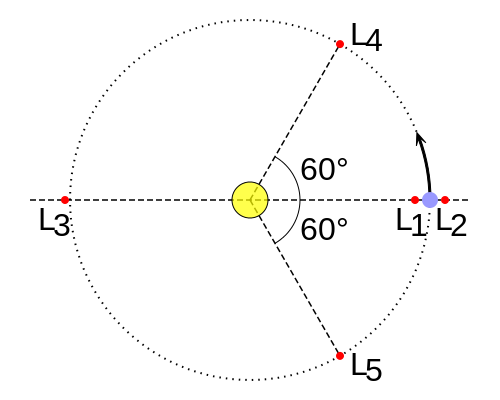
\includegraphics[width=3in]{500px-Lagrange_very_massive.png}
\caption{The trojan points are those labelled L4 and L5, highlighted in red, on the orbital path of the secondary object (blue), around the primary object (yellow).}
\end{figure}



\begin{figure}[H]
\centering
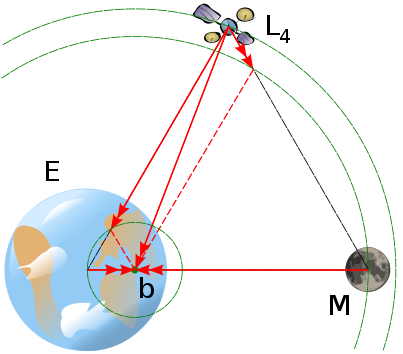
\includegraphics[width=3in]{403px-L4_diagram.png}
\caption{Gravitational accelerations at L4.}
\end{figure}


\begin{figure}[H]
\centering
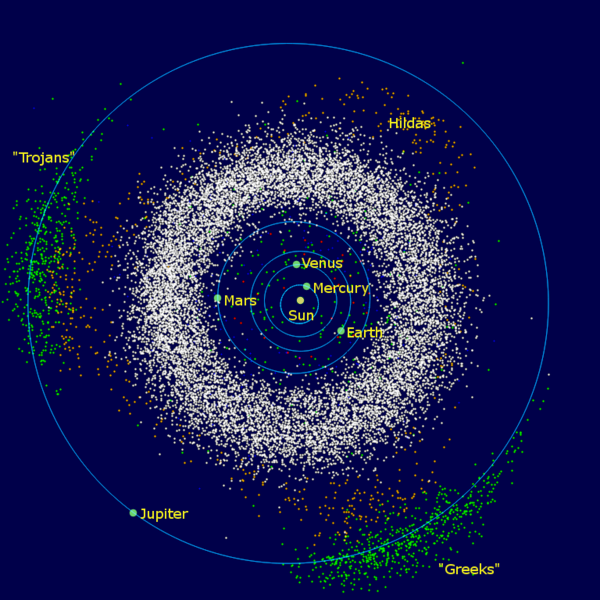
\includegraphics[width=4in]{InnerSolarSystem-en.png}
\caption{The Jupiter trojans in front of and behind the planet along its orbital path, the asteroid belt between Mars and Jupiter, and the Hilda asteroids.The Jupiter trojans are divided into two groups: The Greek camp in front of and the Trojan camp trailing behind Jupiter in their orbit.}
\end{figure}


\begin{figure}[H]
\centering
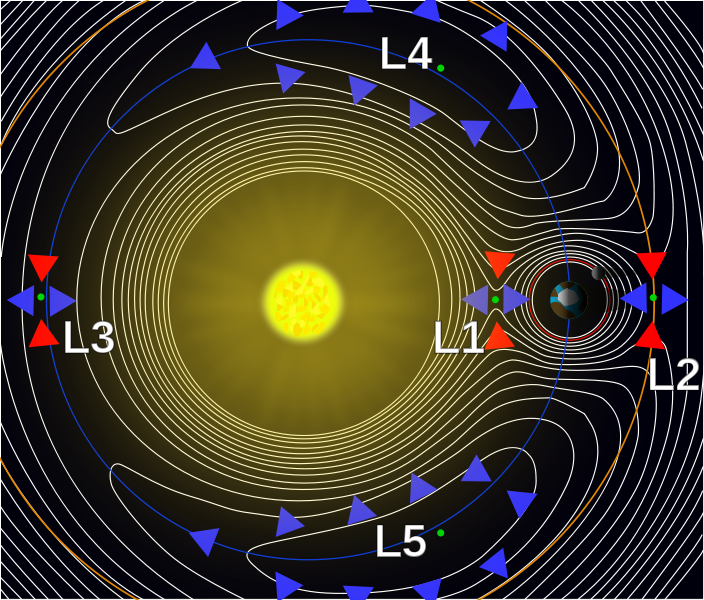
\includegraphics[width=4in]{704px-Lagrange_points2.png}
\caption{A contour plot of the effective potential due to gravity and the centrifugal force of a two-body system in a rotating frame of reference. The arrows indicate the gradients of the potential around the five Lagrange points-downhill toward them (red) or away from them (blue). Counterintuitively, the L4 and L5 points are the high points of the potential. At the points themselves these forces are balanced.}
\end{figure}



\section{Goal and Techniques}

\begin{itemize}
	\item Use adaptive RK4 or Verlet method to simulate the trajectory of a trojan asteroid.
	\item Varying initial conditions in phase space to see if the asteroid are bounded in regions near Lagrangian points. Make a plot of initial conditions which will make bounded motions
	\item  Make a contour plot of gravitational potential near L4 and L5, which determines the range of trojan asteroids. Compare it with the plot made by simulation.
	\item Compare these two plots with Figure 3 which shows the actual positions of Jupiter trojans. Are they different? If so, why?
	\item Vary the ratio of the mass of Sun and planet, to see how the range of trojan asteroids change.
\end{itemize}

\end{document}